% Author: Alexander Svozil
% Matr.-nr.: 1026213
% TU Wien
\documentclass [12pt]{article}
\usepackage [utf8]{inputenc}
\usepackage {graphicx}
\usepackage{algorithm}
\usepackage{algpseudocode}
\usepackage{amssymb}
\usepackage{tikz}
\bibliographystyle{ieeetr} 
\renewcommand{\algorithmicrequire}{\textbf{Input:}}
\newtheorem{mydef}{Definition}

\begin{document}
\author{Alexander Svozil\\ TU Wien}
\title{The Server Location Problem with Restricted Loads 
on Servers and Links}

\maketitle
\newpage

\section{Abstract}
The server location problem with restricted loads on servers and links (SLRL) is an NP-Complete
problem, introduced by Hiroyoshi Miwa et al. in the Paper "Method of Locating Mirror Servers
to Alleviate Load on Servers and Links" \cite{mirrorserver}. The problem 
came up, because the massive volume of data distributed by content delivery networks (CDNs) 
require well located mirror servers in order not to badly influence the quality of their service.
%Two examples for CDNs would be "Amazon CloudFront" a traditional commercial CDN, or the "AT\&T Inc."
%a Telco CDN which has advantages over traditional CDNs because they own the so called "last mile",
%the final leg of the telecommunications networks. CDN nodes are usually deployed in multiple 
%locations, often over multiple backbones, reaching thousands of nodes with tens of thousands of 
%servers. \cite{wiki:cdn} \cite{wiki:lastmile}
The two constraints induced by the choice of mirror servers is the number of maximum nodes
accessing a mirror server and maximum number of nodes accessing a mirror server 
through a specific link. The constraint mentioned first, corresponds to the network load on
the (mirror-)servers. The second constraint corresponds to the restricted load on the links.
First, I will formulate the problem, explain some of the terminology used and prove that SLRL is NP-complete.
Then I will introduce my own algorithm and show performance evaluations comparing the old algorithm proposed 
by Miwa et. al, to my implementation of the tabu search algorithm. 
\newpage
\tableofcontents
\newpage

\section{Introduction}
\subsection {CDNs}
"A content delivery network is a collaborative collection of network elements spanning
the Internet, where content is replicated over several mirrored Web servers in order
to perform transparent and effective delivery of content to the end user."\cite[p. 3]{Buyya:2008:CDN:1457653}\\
"A CDN signs up individual content providers for scalable content delivery and delivers
their content to any client that accesses the Web sites of these content providers."\cite[p. 193]{Rabinovich:2002:WCR:507107}\\
To perform efficient delivery of data, CDNs need to have several mirrored Web servers
and thus it is important to place them well, because placing the mirror server 
could be an expensive choice considering no prior calculation where it should go. 
The expensive choice manifests in high link usages and/or a maximal neighbourhood being
too big for the server to handle. A CDN is able to distribute load among its servers avoid
links that are overused.
The mirror servers naturally serve the same data, as they are there to alleviate the 
load of the other servers providing the data.

\subsection {Similar Problems}
SLRL could be described as an augmented server location problem: 
Two problems that describe this problem would be the p-center and the
p-median problem. The purpose of these problems is mainly to shorten delay
time from the client to the server. 
This class of problems does not care about the maximum load on a link.

\subsubsection {P-Center Problem}
"The P-Center problem consists of locating p facilities and assigning clients
to them in order to minimize the maximum distance between a client and the facility
to which he or she is allocated. It is used for example in locating fire stations or ambulances,
where the distance from the facilities 
to their farthest assigned potential client should be minimum."
The p-center problem is one of the best known NP-hard discrete location problems.
For large instances, it is impractical to solve the problem exactly.
There have been very good results with the tabu-search and variable neighborhood search \cite{Mladenovic00solvingthe}
\cite{KarivHakimi1979}.

\subsubsection {P-Median Problem}
The P-Median Problem is very similar to the P-center problem. It can be defined as follows:
Given a graph G=(V,E) we are asked to find a set of nodes, S, of size p, where $ S\subset V$, such that the weighted
sum of the distances from the remaining nodes \{V-S\} to the Set S is minimized \cite{Rolland1997329}.
This problem belongs to the class of problems known as NP-hard \cite{KarivHakimi1979median}. There have been
approaches to solve this problem with the tabu search \cite{Rolland1997329} and solving the linear program 
\cite{rosing1979p}.


%\subsubsection {NA (Node to Area)-connectivity}
%%TODO: NA-Edge connectivity fehlt:
%\subsection{Open Shortest Path First}
%%TODO: Facility Location with hops
\section{Server Location Problem with Restricted Loads on Servers and Links}
\subsection{Formal Definition}
\subsubsection{Neighbour Set}
The neighbour set is the set of nodes, that belongs to a server. In the SLRL problem, it is
defined as follows: If a non-server node has a shortest path to a server node, he 
belongs to this server nodes neighbour set. If the node has several shortest
paths to multiple server nodes, it belongs to all of the server nodes neighbour
sets. The server itself belongs to its own neighbour set.
\subsubsection{Load on a Link, m(e) or multiplicity of an edge}
The load on a link (edge) is defined as the number of shortest paths, that use this link. If there
are several shortest paths with the same length to one or more servers every
used edge is taken into account. It is mandatory to do this, because we must always consider
the worst case when locating a server. 
\begin{mydef}
  Given a graph G(V,E), and a Set $A= \{ load(e) \ | \ e \in E \}$, m(e) is defined as $e:= max(A)$.
\end{mydef}
\subsubsection{SLRL Problem Definition}

\begin{mydef}
  {\itshape \textbf{Given:} an undirected graph G(V,E) and  positive integers k,r and c.\\
    \textbf{Question:} 
    Is there a subset of Servers S, $S \subseteq V$, where $|S| = k$, $|V|$ $\geq$ k,
    and a subset $|V_i|$ for each Server $s_i \in S$, where $V_i$ is the neighbour set of $s_i$ $(i=1,2,\dots,k)$, r $\geq  |V_i|$ 
  and is $c \geq m(e)$, where m(e) is the maximum load $\forall e \in E$.} 

  %$k = \|S\|$, where S is the set of servers $S = \{s_1,s_2,\dots s_k\} \subseteq V$\\
  %  r $\geq  \|V_i\|$ $(i=1,2,\dots,k)$ where $V_i$ is the neighbour set of $s_i$ $(i=1,2,\dots,k)$\\
  %$c \geq m(e)$, where m(e) is the maximum load $\forall e \in E$.
  %\textbf{Wanted:} 
  %{\itshape A set of Servers $S = \{s_1, s_2,\dots, s_k \} \subseteq V$ such that $|V_i|\leq r$
  %    $(i = 1,2, \dots,k)$ where $V_i$ is the neighbour set of $s_i$  $(i = 1,2,\dots,k)$ and that
  %$m(e) \leq c$ $(\forall e \in E)$.}
\end{mydef}

It is easy to see, that the subset of servers S is a solution to the problem, because the neighborhood subset
of every server can easily be calculated with the graph and the set of servers. Also the load of each edge
can be checked after each shortest path to the server has been looked at (the maximum is m(e)).

\subsection{An Instance Of The Problem}
\indent
\indent
\indent

\includegraphics [scale=0.23]{cableandwireless1.png}\\
The above shown graph is from the barebone network "Cable and Wireless".
It is parsed out of a dataset of barebone networks provided by caida.\cite{caidabarebones}
\\
The nodes have two values in their bubbles: "NH and m(e)". NH stands for 
the maximum neighbourhood if that node was chosen as a server. Choosing the first
server obviously implicates the maximum neighbourhood, because there are
no mirror servers yet on the graph.\\
The multiplicity of an edge e, $m(e)$ is explained above. The number after
$m(e)$ in the bubble describes $max(m(e))$ $ \forall e \in E$,
if one decides to take this node as a server.
The greedy algorithm takes the node with the lowest $max(m(e))$ first.
\\
\includegraphics [scale=0.23]{cableandwireless2.png}\\
This graph shows the second server pick. This time our $m(e)$ is already low enough
to suffice the constraint $m(e)\leq c $ thus the greedy algorithm proposed in the paper 
by Miwa et al. \cite{mirrorserver} chooses the node with the lowest max neighbourhood which is
coincidentally also the one with the lowest $m(e)$.


\subsection{Proof of NP-Completeness}
First, we have to show that SLRL is in NP. After guessing a solution of servers, meaning we 
have an instance of SLRL (G,r,c,k) and a guessed set of servers S, one can clearly check 
in polynomial time whether it is a valid solution for SLRL: We need to check that every neighbor set is smaller
or equal to r. Also the number of servers have to be k and the maximum usage of every edge may not exceed c.
Calculating every neighbor set is done with breadth-first search: Every vertex that is not a server calculates
the path to every server and marks the path so the usage gets tracked. This is in $\mathcal{O}(V*(V+E)*S)$, as breadth first
search is in $\mathcal{O}(V+E)$. Checking the set for size is also trivial as is looking at the usage of
every edge and comparing the maximum with c.\\
After proving that SLRL is in NP, it can be shown, that 3SAT can be reduced to SLRL in polynomial time,
implying SLRL is NP-Complete \cite{Garey:1979:CIG:578533}.
This proof is merely a rewriting of Miwa et al. \cite{mirrorserver}, as it is one of the first proofs I saw of 
this kind, it was really interesting for me to figure it out.
3SAT is like the satisfiability problem for arbitrary formulars, but in 3SAT the formula must be in KNF and 
each clause may only consist of three literals. A solution for 3SAT would be a truth assignment to every
variable. An instance of 3SAT (U,C) consists of a set of clauses C and a set of variables U.\\
To reduce 3SAT to SLRL, and thus to prove that SLRL is at least as hard as 3SAT, we need to find a 
transformation $R: x \rightarrow y$ where $x \in 3SAT$ and $y \in SLRL$. This transformation must be 
done in polynomial time. After the transformation, we need to show that 3SAT has a solution if and only if 
SLRL has a solution.\\
The steps to construct an instance of SLRL (G=(V,E),k,r,c) of an instance of 3SAT (U,C) are described below.
\begin{enumerate}
  \item{Let V $\leftarrow \emptyset$ and E $\leftarrow \emptyset$.}
  \item{For each $C_i \in C$ where (i = 1,\dots,m), let $c_i$ be a vertex, and for each $u_j \in U$ for (j = 1,\dots,n),
    let $t_j$ and $f_j$ be a vertex.}
  \item {Let V $\leftarrow \{c_1, \dots, c_m\} \cup \{t_1, \dots, t_n, f_1, \dots, f_n\} $ }
  \item {Let E $\leftarrow \{(t_i,f_i)\}$ for (i = 1,\dots,n) }
  \item {For each $C_i \in C$ for (i = 1,\dots,m), if $u_j \in C_i$, let E $\leftarrow$ E $\cup \ \{ (c_i ,t_j) \}$
    and if $\neg u_j \in C_i$, let E $\leftarrow$ E $\cup \ \{(c_i,f_j)\}$ }
  \item{For each (i=1,\dots,m) and (j=1,\dots,n) let V $\leftarrow$  V $\cup \ \{v_{ij}\}$ and E $\leftarrow$ E $\cup \ \{(t_i,v_{ij}), (f_i, v_{ij} \}$ }
  \item{Let k = n, r = 2m+2 and c = 1}
\end{enumerate}
\begin{figure}[h!]
  \centering
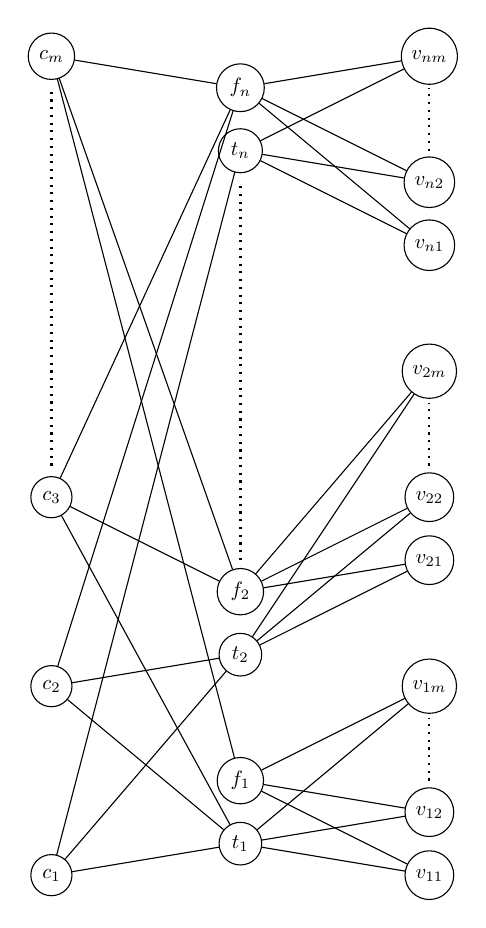
\begin{tikzpicture}
  [scale=0.8,auto=left,every node/.style={circle, draw, scale=0.75}]
  \node (c1) at (1,0) {$c_1$};
   \node (t1) at (4,0.5) {$t_1$};
   \node (f1) at (4,1.5) {$f_1$};
   \node (v11) at (7,0) {$v_{11}$};
   \node (v12) at (7,1) {$v_{12}$};
   \node (v1m) at (7,3) {$v_{1m}$};
  \node (c2) at (1,3) {$c_2$};
   \node (t2) at (4,3.5) {$t_2$};
   \node (f2) at (4,4.5) {$f_2$};
     \node (v21) at (7,5) {$v_{21}$};
     \node (v22) at (7,6) {$v_{22}$};
     \node (v2m) at (7,8) {$v_{2m}$};

  \node (c3) at (1,6) {$c_3$};
  \node (cm) at (1,13) {$c_m$};

   \node (tn) at (4,11.5) {$t_n$};
   \node (fn) at (4,12.5) {$f_n$};
     \node (vn1) at (7,10) {$v_{n1}$};
     \node (vn2) at (7,11) {$v_{n2}$};
     \node (vnm) at (7,13) {$v_{nm}$};
  
  \draw[dotted,thick] (1,6.5) -- (1,12.5);
  \draw[dotted,thick] (4,5) -- (4,11);
  \draw[dotted,thick] (7,1.5) -- (7,2.5);
  \draw[dotted,thick] (7,6.5) -- (7,7.5);
  \draw[dotted,thick] (7,11.5) -- (7,12.5);

  \foreach \from/\to in {c1/t1, c1/t2, c1/tn, c2/t1, c2/t2, c2/fn, c3/t1, c3/f2, c3/fn, cm/f1, 
  cm/f2, cm/fn, 
  v11/t1, v11/f1, v12/t1, v12/f1, v1m/t1, v1m/f1,
  v21/t2, v21/f2, v22/t2, v22/f2, v2m/t2, v2m/f2,
  vn1/tn, vn1/fn, vn2/tn, vn2/fn, vnm/tn, vnm/fn}
      \draw (\from) -- (\to);
\end{tikzpicture}
  \caption{The transformation from 3SAT to SLRL}
\end{figure}
Now it must be proven, that 3SAT has a solution if and only if SLRL has a solution. 
To prove the statement, it will be first shown, that if 3SAT has a Solution SLRL has a solution.
\begin{enumerate}
  \item{Assume 3SAT has a solution, that means we have a truth assignment, 
    which satisfies all the clauses.}
  \item{Construct the set of servers S as follows: If variable $u_j \in U$ is true
      in the truth assignment, then add $t_j$ to the server set. If variable $u_j \in U$
      is false, then add $f_j$ to the server set. Do this for each variable $u_j$ for $j = (1,\dots,n)$.
      As there are exactly n variables in U, this clearly satisfies our constraint 
    for k, i.e., the number of servers.}
  \item{At most m clauses inherit the variable $u_j$. There are m vertices connected to every
      $t_j$ and $f_j$, i.e., $v_{ij}$ for $i=(1,\dots,m)$.
      Thus the number of vertices in the neighbor set is $m+m+2 = 2m+2 \leq r $ for every 
      $t_j$ or $f_j$. The additional two vertices result of the server and the respective 
    vertex representing the other truth value.}
  \item{The usage of each edge is one, which means it is smaller and equal to c. $1\leq c$.
    Thus it is obvious that this constraint is not violated.}

  \item{Consequently this instance of SLRL, (G,k,r,c) has a solution, because all constraints are satisfied 
    and as a result the first part of the equivalence is proved.}
\end{enumerate}
To finish our prove we need to show the converse, i.e., 
if (G,k,r,c) is a solution there is a solution for 3SAT aswell. 

\begin{enumerate}
  \item{Assume (G,k,r,c) has a solution. Let $G_i, (i=1,\dots,n)$ be the subgraph induced
    by $t_i, f_i$ and $v_{ij},(j=1,\dots,m)$.}
  \item{We will now show, that there is only one way to place the servers, namely the truth
    value assignment for the variables, that satisfy the 3SAT instance}
  \item{Assume that there is no server in $G_i$. This would imply that the servers is a subset of
      $c_j for j=(1..m)$. The problem there is, that not only is m != n(concerning constraint k),
      but also that constraint c would be unsatisfied, because more than one path would use 
      the edge connecting $c_j$ and either $f_i$ or $t_i$ (there are m + 2 vertices in $G_i$).
    Thus placing a server on any $c_j$ is not possible, because it would automatically violate contraint c.}
  \item{Assume that the servers are placed on $v_{ij}$. This would also satisfy the neighborhood 
      constraint r, but it would certainly violate the constraint c, because the degree of $v_{ij}$ is two and
      and the number of vertices in $G_i$ is m+2. All of them would need to use one of the two edges for their shortest path,
    resulting in a violation.}
  \item{The only spare option that would satisfy the neighborhood constraint 
      are the vertices $t_i$ and $f_i$. Let $u_i$ be true if a server is located on
      $t_i$ and let $u_i$ be false if a server is located on $f_i$. Now this would not yet 
      guarantee a solved 3SAT instance nor a solution of the SLRL because we need to put
      the servers on the right spots. If a $c_j$ has no adjacent vertices which are servers,
      the SLRL would not be fulfilled because there would be two shortest paths passing edge
      $(t_i,f_i)$. This would contradict $c = 1$. Therefore, the truth assignments satisfy all
    clauses.}
\end{enumerate}
Thus 3SAT was successfully reduced to SLRL in polynomial time.
Consequently, SLRL is NP-complete.$\square$
\section{Algorithm}
\subsection{Rules and Assumptions}
\subsection{Other Algorithms}
The only prior algorithm for this problem is the greedy algorithm proposed by
Miwa et al. \cite{mirrorserver}. It greedily chooses the node with the 
lowest maximal neighbourhood if the constraint $c\geq m(e) (\forall e \in E)$ is fulfilled. 
Otherwise it will choose a node where $min(m(e)(\forall e \in E))$ is true.


\subsection{Data (Testinstances)}
The data taken for the tests is from caida \cite{caidabarebones}. Parsing the
data was one of the most difficult parts, because the data is not formatted well.
It does not really follow the syntax proposed in the beginning of the file. I also
modified the data in some concerns:
\begin{itemize}
  \item If the graph G given for the barebone network was not connected,
    the connected component with less nodes of that graph is cut out.

  \item Normally the connected cities are listed in this manner:
    "city,state,country", in order to match with the numbers 
    in the paper \cite{mirrorserver} only city and state are used for
    identification and the country is left out. Sometimes London
    is used on one hand as City in Canada and on the other hand in GB, denoted like this
    London, *, Canada and London, *, England. They are differentiated.
  \item Sometimes the State has a number. One example would be "Kansas City, KS2~"
    This is interpreted as "Kansas City, KS".

\end{itemize}

All those modifications were done to match the graphs proposed by \cite{mirrorserver}.
As I did not have the data of the other paper used, I tried to match them with the number of
nodes and number of vertices. Unfortunately three instances of my instances do not
match the number of nodes and / or vertices proposed from the paper above.
The varying instances are: "Sprint", "Cable and Wireless" and "UUNet".

\section{Implementation}
I decided to implement a tabu-search.
\subsection{Determination of the neighbour sets of a server and loads of the links}
When a server is added to the graph, r and $max(m(e))$ $\forall e\in E $ need to be recalculated, as the shortest paths from the clients
to the servers change. This has to be done for every client in order to ensure that every client has its path(s) and server(s).
The outer loop goes through every n that is not a server and tests out every server if it is the closest. There can be more than one 
closest server. It will be saved in the nearestServersList. The path to the server is then marked. If there is a new nearest Server, these
stats are reset and the newly found nearest servers edges are marked.
It takes $\mathcal O(|V|-|S| * |S| * |V+E|^2 ) $ to calculate the new r and the new $max(m(e))$ $\forall e\in E$, as BFS costs $ \mathcal O(|V| + |E|) $
and backtracking every path can also result in visiting every node and every edge and thus costs $\mathcal O(|V| + |E|)$.
\begin{algorithm}[H]
  \caption{constraintsCalculation}
  \begin{algorithmic}[2]
    \Require Graph (V,E) G, Servers S
    \For{Each node n $\in G$}
    \If{!($n \in S$)}
    \State $nearestServersList \gets \{\};$ 
    \State $minServer \gets 0;$ \Comment The stepcounter to the nearest server(s)
    \For {Each Server $ s \in S$}
    \State $BFS2(n,s)$
    \State $p \gets s;$
    \State $i \gets s.getDistance() $ \Comment distance to server acquired in BFS 
    \If {$i \leq minServer || nearestServersList.isEmpty()$}
    \If {$i < minServer$}
    \For{Each Server prevNearest $\in nearestServersList$}
    \State $prevnearest.tmpNeighbourhood=0;$
    \State $nearestServersList.clear();$
    \State $usedEdges.clear();$
    \EndFor
    \EndIf
    \State $minServer = i;$ \Comment new nearest server found, set length
    \State $nearestServersList.add(s);$ \Comment add it to the list of nearest servers 
    \State $s.tmpNeighbourhood += 1;$ \Comment adds one to the temporal neighbourhood (it may get reset later on)
    \State $markPath2(s)$ \Comment This method recusively walks back every node's parents list to determine every path and add it to the usedEdges list.
    \EndIf 
    \EndFor
    \For{Each Server s $\in nearestServerList$}
    \State $s.neighborhood += s.tmpNeighbourhood;$
    \State $s.tmpNeighbourhood = 0;$
    \EndFor
    \State $markEdges();$ \Comment increments usage of each usedEdges
    \EndIf
    \EndFor
  \end{algorithmic}
\end{algorithm}
\subsection{Modified BFS}
The Breadth first search needed to be modified in order for it to be able to find all shortest paths
from one node to another, as we need to consider every shortest path in order to simulate
the worst case scenario regarding load on links. It's runtime $\mathcal O(|V| + |E|)$ remains unmodifed.

\begin{algorithm}[H]
  \caption{BFS2}
  \begin{algorithmic}[2]
    \Require Graph(V,E) G, Node dest, Node start
    \State $clearParents();$
    \State $resetDistance();$
    \State Queue$<$Node$>$ nodeQueue $\gets \{\};$
    \State Set$<$Node$>$ visited $\gets \{\};$
    \State $visited.add(start);$
    \State $nodeQueue.offer(start);$ \Comment \begin{itshape} Nodepair saves the node and the parentnode,
    so all the paths can be reconstructed\end{itshape}
    \While {$!nodeQueue.isEmpty()$}
  \State $Node$ $curNode$ $=$ $nodeQueue.poll();$ \Comment \begin{itshape} get first node out of queue\end{itshape}
  \State $visited.add(curNode);$ \Comment \begin{itshape} mark node as visited\end{itshape}            
    \If{$!curNode.equals(dest)$}
    \State {$return$ $dest;$}
    \EndIf
    \For{$Edge$ $e$ : $curNode.getEdges()$}
    \If{$!visited.contains(e.getNode2())$}
    \If{$e.getNode2().getDistance() == curNode.getDistance() + 1 \| e.getNode2().getDistance() == -1$}
    \State $alreadyVis \gets false;$
    \For{$Node$ $node$ : $nodeQueue$}
    \State $node.addParent(curNode);$
    \State $alreadyVis \gets true;$
    \State $break;$
    \EndFor
    \If{$!alreadyVis$}
    \State $nodeQueue.offer(e.getNode2());$
    \State $e.getNode2().addParent(curNode);$
    \State $e.getNode2().setdistance(curNode.getDistance()+1);$
    \EndIf
    \EndIf
    \EndIf
    \EndFor
    \EndWhile
  \end{algorithmic}
\end{algorithm}
\subsection{The local search}
The Local search simply exchanges a server with a client and recalculates the constraints to create a neighborhood N of feasible solutions.

\begin {algorithm} [H]
\caption {localsearch}
\begin {algorithmic} [3]
\Require Graph(V,E), Set
\end {algorithmic}
\end {algorithm}
\subsection{The tabu-search}
\subsection{Networks and the approximation ratio}
\section{Performance Evaluation}
  \begin{tabular}{ | l | l | l | l | l | l | l | l | l |  }
    \hline
    Networks & n & m &\# of Servers & r* & r & r/r* & c & m(c) \\ \hline
    above.net & 22 & 25 & 3 & 8 & 13 & 1.625 & 3 & 3\\ \hline
    At Home Network & 46 & 55 & 5 & 10 & 13 & 1.1 & 8 & 7\\ \hline
    AGIS & 82 & 92 & 9 & 10 & 15 & 1.1 & 10 & 7\\ \hline
    AT\&T WorldNet & 93 & 154 & 10 & 10 & 28 & 4.3 & 2 & 4\\ \hline
    BBN Planet & 41 & 49 & 5 & 9 & 13 & 1.44 & 5 & 4\\ \hline
    Cable Internet & 8 & 7 & 1 & 8 & 8 & 1.0 & 8 & 4\\ \hline
    CAIS Internet & 37 & 44 & 4 & 10 & 12 & 1.1 & 10 & 7\\ \hline
    CompuServe Network Services & 16 & 23 & 2 & 8 & 11 & 1.375 & 5 & 3\\ \hline
    CRL Network Services & 35 & 50 & 4 & 9 & 21 & 1.44 & 4 & 4\\ \hline
    DataXchange Network, Inc. & 8 & 24 & 1 & 8 & 8 & 1.0 & 5 & 1\\ \hline
    Allegiance Telecom & 53 & 88 & 6 & 9 & 26 & 2.888 & 3 & 4\\ \hline
    EPOCH Networks, Inc. & 29 & 30 & 3 & 10 & 14 & 1.4 & 6 & 6\\ \hline
    EUnet & 28 & 30 & 3 & 10 & 23 & 2.3 & 2 & 2\\ \hline
    Exodus & 14 & 19 & 2 & 7 & 9 & 1.285 & 4 & 3\\ \hline
    Genuity & 48 & 53 & 5 & 10 & 12 & 1.3 & 8 & 8\\ \hline
    GeoNet Communications, Inc. & 13 & 15 & 2 & 7 & 11 & 1.571& 3 & 1\\ \hline
    GetNet International & 5 & 6 & 1 & 5 & 5 & 1.0 & 7 & 2\\ \hline
    GlobalCenter & 9 & 36 & 1 & 9 & 9 & 1.0 & 5 & 1\\ \hline
    GoodNet & 27 & 58 & 3 & 9 & 20 & 2.223 & 2 & 2\\ \hline
    IDT Corp & 15 & 18 & 2 & 8 & 10 & 1.25 & 6 & 4\\ \hline
    ipf.net & 5 & 5 & 1 & 5 & 5 & 1.0 & 7 & 2\\ \hline
    iSTAR Internet Inc. & 20 & 22 & 2 & 10 & 14 & 1.4 & 6 & 6\\ \hline
    Cable \& Wireless & 20 & 34 & 2 & 10 & 14 & 1.3 & 7 & 7\\ \hline
    MindSpring & 41 & 45 & 5 & 9 & 22 & 2.44 & 2 & 2\\ \hline
    Nap.Net, LLC & 6 & 7 & 1 & 6 & 6 & 1.0 & 5 & 1\\ \hline
    Netrail Incorporated & 17 & 21 & 2 & 9 & 12 & 1.33 & 6 & 3\\ \hline
    PSINet & 78 & 110 & 8 & 10 & 20 & 1.8 & 5 & 5\\ \hline
    Qwest & 14 & 26 & 2 & 7 & 9 & 1.285 & 4 & 2\\ \hline
    RISQ Network & 13 & 12 & 2 & 7 & 8 & 1.142 & 4 & 2\\ \hline
    RNP & 27 & 35 & 3 & 9 & 12 & 1.333 & 3 & 2\\ \hline
    Savvis Communications & 28 & 56 & 3 & 10 & 20 & 2.0 & 4 & 4\\ \hline
    ServInt Internet Services & 23 & 34 & 3 & 8 & 11 & 1.375 & 5 & 5\\ \hline
    Sprint & 21 & 37 & 3 & 7 & 12 & 1.428 & 4 & 3\\ \hline
    Telstra Internet & 21 & 24 & 3 & 7 & 13 & 1.857 & 2 & 2\\ \hline
    UUNET & 126 & 316 & 13 & 10 & 29 & 2.9 & 2 & 6\\ \hline
    Verio & 35 & 72 & 4 & 9 & 19 & 2.0 & 3 & 3\\ \hline
    VisiNet & 11 & 13 & 2 & 6 & 7 & 1.1666 & 4 & 2\\ \hline
    XO Communications & 33 & 38 & 4 & 9 & 16 & 1.333 & 5 & 5\\ \hline
  \end{tabular}
\section{Conclusion}

\bibliography{bibtex}
\end{document}
